%! Unidad 7 — Física cuántica (teoría, actividades resueltas y prácticas)
%! Fuente: Fuentes/Tema_7.pdf (reescrito; datos de las actividades cambiados y recalculados)

\section*{Para empezar: dos nubecillas en el horizonte}
\addcontentsline{toc}{section}{Para empezar: dos nubecillas en el horizonte}

En 1900, Lord Kelvin dijo en una conferencia que la física estaba prácticamente terminada: la mecánica de Newton y el
electromagnetismo de Maxwell lo explicaban casi todo. Solo quedaban «dos nubecillas en el horizonte»: el resultado negativo de un
experimento que buscaba el éter y la forma en que brillan los cuerpos calientes. Aquellas dos nubecillas dieron lugar a las dos
grandes teorías del siglo \textsc{xx}: la \textbf{relatividad} y la \textbf{física cuántica}. Gracias a la segunda entendemos cómo
funcionan los átomos, los láseres, los LED, las placas solares o los chips de un teléfono móvil. En esta unidad veremos los
experimentos que obligaron a abandonar la física clásica y las ideas, a veces sorprendentes, que la sustituyeron.

\section{Las ondas electromagnéticas}\label{sec:cua-espectro}

Una carga eléctrica acelerada emite energía en forma de \rojon{onda electromagnética}: un campo eléctrico y un campo magnético
que oscilan perpendiculares entre sí y a la dirección de propagación (figura~\ref{fig:cua-onda}). Son ondas transversales que no
necesitan medio material y que, en el vacío, viajan a \(c = \qty{3e8}{\m\per\second}\). Como toda onda, cumplen \(c = \lambda\nu\).

\begin{figure}[H]
    \centering
    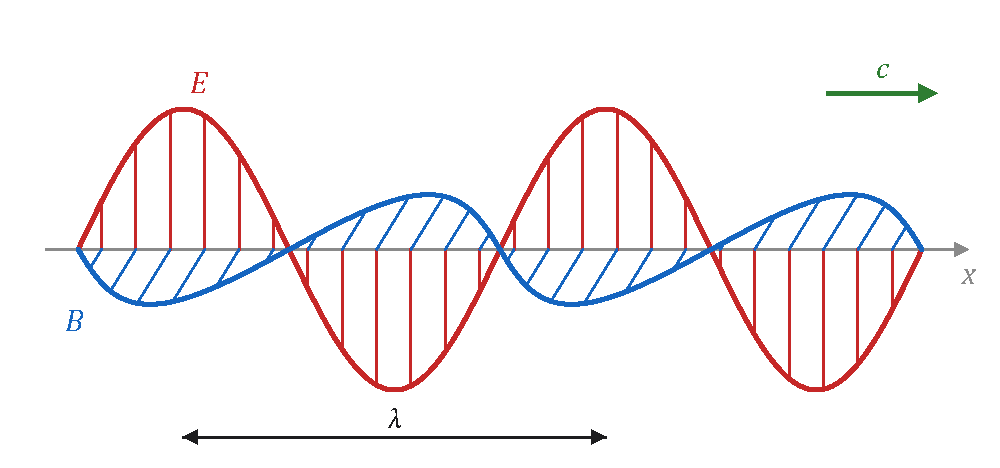
\includegraphics[width=0.66\linewidth]{images/UD7/onda_em}
    \caption{En una onda electromagnética \(\vec E\) y \(\vec B\) oscilan en fase, perpendiculares entre sí y a la propagación.}
    \label{fig:cua-onda}
\end{figure}

El \rojon{espectro electromagnético} es el conjunto de todas las ondas electromagnéticas, ordenadas según su frecuencia
(figura~\ref{fig:cua-espectro}):
\begin{itemize}
    \item \textbf{Ondas de radio} (hasta \qty{e9}{\hertz}): radio, televisión. Se producen con corrientes oscilantes en antenas.
    \item \textbf{Microondas} (\qtyrange{e9}{e11}{\hertz}): radar, telefonía móvil, wifi, hornos de microondas.
    \item \textbf{Infrarrojo} (\qtyrange{e11}{4e14}{\hertz}): lo emiten los cuerpos calientes; mandos a distancia, cámaras térmicas.
    \item \textbf{Luz visible} (\qtyrange{4e14}{7.5e14}{\hertz}, de \qty{750}{\nm} a \qty{400}{\nm}): del rojo al violeta.
    \item \textbf{Ultravioleta} (\qtyrange{7.5e14}{e17}{\hertz}): broncea la piel y puede dañarla; esteriliza.
    \item \textbf{Rayos X} (\qtyrange{e17}{e19}{\hertz}): radiografías.
    \item \textbf{Rayos gamma} (más de \qty{e19}{\hertz}): los emiten los núcleos radiactivos; radioterapia.
\end{itemize}

\begin{figure}[H]
    \centering
    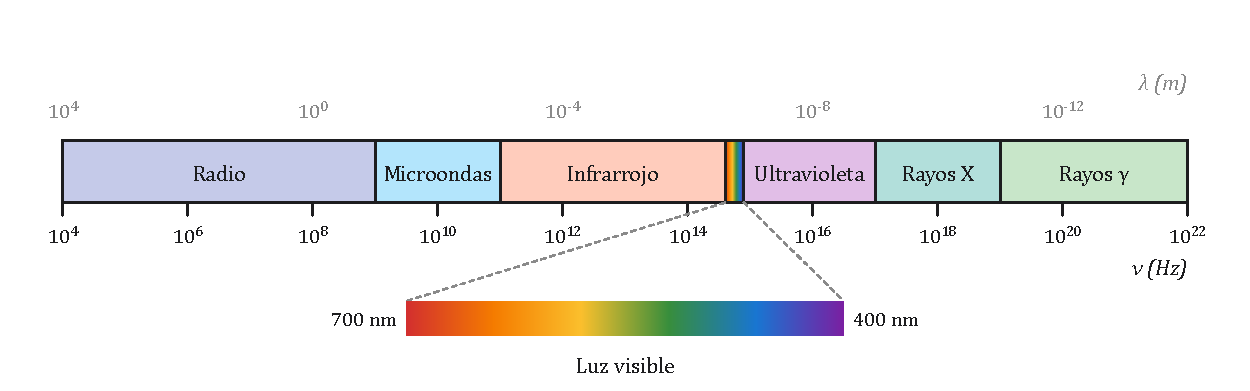
\includegraphics[width=0.95\linewidth]{images/UD7/espectro}
    \caption{El espectro electromagnético. La luz visible es una franja estrechísima.}
    \label{fig:cua-espectro}
\end{figure}

\section{La radiación del cuerpo negro}\label{sec:cua-cuerpo-negro}

Todos los cuerpos emiten radiación electromagnética por estar a una temperatura: es la \azuln{radiación térmica}. A temperatura
ambiente es casi toda infrarroja e invisible; al calentar un trozo de hierro, empieza a brillar rojo, luego amarillento y, a muy
alta temperatura, casi blanco.

Para estudiarla se usa un modelo ideal, el \rojon{cuerpo negro}: un cuerpo que absorbe toda la radiación que le llega y que, por
tanto, emite radiación de todas las longitudes de onda, con un espectro que solo depende de su temperatura. Una buena aproximación
es una cavidad con un pequeño orificio: la radiación que entra queda atrapada tras varias reflexiones (figura~\ref{fig:cua-cavidad}).

\begin{figure}[H]
    \centering
    \begin{minipage}[b]{0.34\linewidth}
        \centering
        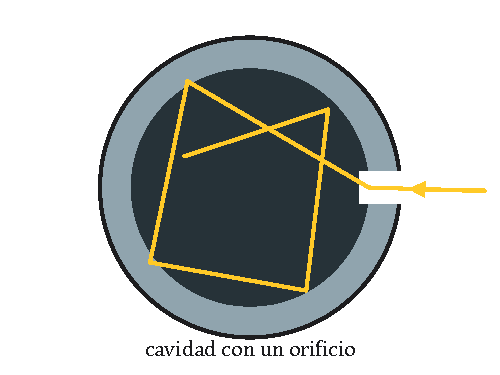
\includegraphics[width=\linewidth]{images/UD7/cuerpo_negro}
        \caption{Cavidad que actúa como cuerpo negro.}
        \label{fig:cua-cavidad}
    \end{minipage}\hfill
    \begin{minipage}[b]{0.62\linewidth}
        \centering
        \begin{tikzpicture}
            \begin{axis}[fisica, width=\linewidth, height=5.2cm, xmin=0, xmax=3.1, ymin=0, ymax=1.15,
                xlabel={\(\lambda\) (\unit{\micro\m})}, ylabel={\(I\)}, xtick={0.5,1,1.5,2,2.5,3}, ytick=\empty, samples=120,
                legend style={font=\scriptsize, draw=none, at={(0.98,0.95)}, anchor=north east}]
                \addplot[domain=0.12:3, very thick, red] {(1/(x^5*(exp(14.388/(x*5))-1)))/0.1075};
                \addlegendentry{\qty{5000}{\kelvin}}
                \addplot[domain=0.12:3, very thick, ocre] {(1/(x^5*(exp(14.388/(x*4))-1)))/0.1075};
                \addlegendentry{\qty{4000}{\kelvin}}
                \addplot[domain=0.12:3, very thick, blue] {(1/(x^5*(exp(14.388/(x*3))-1)))/0.1075};
                \addlegendentry{\qty{3000}{\kelvin}}
                \addplot[domain=1.32:3, thick, dashed, gray] {5/(14.388*x^4)/0.1075};
                \node[font=\scriptsize, gray, anchor=west] at (axis cs:1.4,1.08) {Rayleigh-Jeans (5000 K)};
            \end{axis}
        \end{tikzpicture}
        \caption{Espectro del cuerpo negro (ley de Planck). La predicción clásica (discontinua) se dispara a longitudes de onda cortas.}
        \label{fig:cua-planck}
    \end{minipage}
\end{figure}

Las medidas experimentales llevaron a dos leyes:
\begin{itemize}
    \item \textbf{Ley de Wien}. La longitud de onda a la que la emisión es máxima es inversamente proporcional a la temperatura
    absoluta:
    \begin{centeredequation}
        \boxed{\lambda_{\text{máx}}\,T = b} \qquad b = \qty{2.9e-3}{\m\kelvin} \label{eq:cua-wien}
    \end{centeredequation}
    Por eso las estrellas más calientes son azuladas y las más frías, rojizas.
    \item \textbf{Ley de Stefan-Boltzmann}. La potencia emitida por unidad de superficie es proporcional a la cuarta potencia de la
    temperatura absoluta:
    \begin{centeredequation}
        \boxed{I = \sigma\,T^4} \qquad \sigma = \qty{5.67e-8}{\watt\per\m\squared\per\kelvin\tothe{4}} \label{eq:cua-stefan}
    \end{centeredequation}
\end{itemize}

\paragraph{La catástrofe ultravioleta.} Rayleigh y Jeans intentaron explicar el espectro con la física clásica, suponiendo que los
átomos de las paredes oscilan y emiten energía de forma continua. Su fórmula, \(I \propto T/\lambda^4\), funcionaba bien a longitudes de
onda largas, pero predecía que la intensidad crecería sin límite al acercarse al ultravioleta: un cuerpo caliente emitiría una
energía infinita. Este fracaso se llamó \azuln{catástrofe ultravioleta} (figura~\ref{fig:cua-planck}).

\section{La hipótesis de Planck}\label{sec:cua-planck}

En 1900, Max Planck encontró una fórmula que se ajustaba perfectamente a las medidas. Para justificarla tuvo que hacer una suposición
revolucionaria, que él mismo consideró un «acto de desesperación»:

\begin{definition}[Hipótesis de Planck]
    La energía de los osciladores que emiten radiación no puede tomar cualquier valor: solo puede emitirse o absorberse en paquetes,
    los \rojon{cuantos}, cuya energía es proporcional a la frecuencia:
    \begin{centeredequation}
        \boxed{E = h\,\nu = \dfrac{h\,c}{\lambda}} \label{eq:cua-planck}
    \end{centeredequation}
    donde \(h = \qty{6.63e-34}{\joule\second}\) es la \azuln{constante de Planck}.
\end{definition}

La energía está \textbf{cuantizada}: un oscilador solo puede tener energías \(h\nu\), \(2h\nu\), \(3h\nu\)\ldots{} Como \(h\) es
tan pequeña, en el mundo cotidiano los saltos son imperceptibles y la energía parece continua. Es habitual expresar estas energías en
\azuln{electronvoltios}: \(\qty{1}{\electronvolt} = \qty{1.6e-19}{\joule}\), la energía que gana un electrón al acelerarse con una
diferencia de potencial de \qty{1}{\volt}.

\begin{exercise}
    Calcula, en julios y en electronvoltios, la energía de un fotón de una emisora de FM de \qty{95}{\mega\hertz}.
    \begin{solu}
        \(E = h\nu = 6{,}63\cdot 10^{-34}\cdot 95\cdot 10^6 = \textcolor{red}{\qty{6.30e-26}{\joule}}\) \(= \dfrac{6{,}30\cdot 10^{-26}}{1{,}6\cdot 10^{-19}} = \textcolor{red}{\qty{3.94e-7}{\electronvolt}}\).
    \end{solu}
\end{exercise}

\begin{exercise}
    El espectro visible va de \qty{400}{\nm} a \qty{750}{\nm}. ¿Entre qué energías, en eV, están sus fotones?
    \begin{solu}
        \(E = \dfrac{hc}{\lambda}\): \(E_{400} = \dfrac{6{,}63\cdot 10^{-34}\cdot 3\cdot 10^8}{400\cdot 10^{-9}\cdot 1{,}6\cdot 10^{-19}} = \textcolor{red}{\qty{3.11}{\electronvolt}}\);
        \(E_{750} = \textcolor{red}{\qty{1.66}{\electronvolt}}\).
    \end{solu}
\end{exercise}

\begin{exercise}
    El filamento de una bombilla está a \qty{2027}{\celsius}. ¿A qué longitud de onda emite con más intensidad? ¿Por qué estas bombillas
    calientan tanto?
    \begin{solu}
        \(\lambda_{\text{máx}} = \dfrac{b}{T} = \dfrac{2{,}9\cdot 10^{-3}}{2300} = \textcolor{red}{\qty{1261}{\nm}}\):
        \textcolor{red}{en el infrarrojo}. \textcolor{blue}{La mayor parte de la energía sale como calor y solo una pequeña parte como luz visible.}
    \end{solu}
\end{exercise}

\begin{exercise}
    Un cuerpo caliente emite con una potencia de \qty{0.05}{\watt} radiación cuyo máximo está en \qty{650}{\nm}. Suponiendo que toda
    fuera de esa longitud de onda, ¿cuántos fotones emite en un minuto?
    \begin{solu}
        \textcolor{blue}{Energía de cada fotón: \(E = hc/\lambda = \qty{3.06e-19}{\joule}\). Energía emitida en un minuto: \(0{,}05\cdot 60 = \qty{3}{\joule}\).}
        \(N = \dfrac{3}{3{,}06\cdot 10^{-19}} = \textcolor{red}{\num{9.8e18}\ \text{fotones}}\).
    \end{solu}
\end{exercise}

\begin{exercise}
    La superficie del Sol está a unos \qty{5800}{\kelvin}. ¿A qué longitud de onda emite con más intensidad? ¿Qué potencia emite por
    cada metro cuadrado?
    \begin{solu}
        \(\lambda_{\text{máx}} = \dfrac{2{,}9\cdot 10^{-3}}{5800} = \textcolor{red}{\qty{500}{\nm}}\) \textcolor{blue}{(en el centro del visible)};
        \(I = \sigma T^4 = 5{,}67\cdot 10^{-8}\cdot 5800^4 = \textcolor{red}{\qty{6.4e7}{\watt\per\m\squared}}\).
    \end{solu}
\end{exercise}

\section{El efecto fotoeléctrico}\label{sec:cua-fotoelectrico}

El \rojon{efecto fotoeléctrico} es la emisión de electrones por un metal cuando se ilumina con luz de frecuencia adecuada. Se
estudia con un tubo de vacío que contiene una placa metálica (el cátodo) y otra que recoge los electrones (el ánodo), conectadas a una
fuente de tensión regulable (figura~\ref{fig:cua-fotoelectrico}). Al iluminar el cátodo, el amperímetro marca corriente.

\begin{figure}[H]
    \centering
    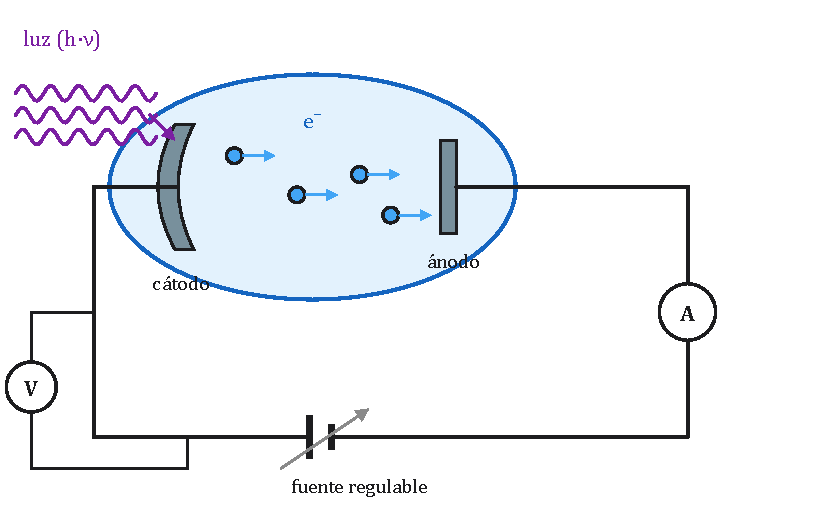
\includegraphics[width=0.55\linewidth]{images/UD7/fotoelectrico}
    \caption{Montaje para estudiar el efecto fotoeléctrico.}
    \label{fig:cua-fotoelectrico}
\end{figure}

Los resultados experimentales eran:
\begin{enumerate}[label=\numberballmDarkTeal]
    \item Para cada metal hay una \azuln{frecuencia umbral} \(\nu_0\): con luz de frecuencia menor no se emiten electrones, \emph{por
    intensa que sea}.
    \item Por encima del umbral, la emisión es instantánea, aunque la luz sea muy débil.
    \item La energía cinética máxima de los electrones depende de la frecuencia de la luz, no de su intensidad.
    \item El número de electrones emitidos (la intensidad de la corriente) es proporcional a la intensidad de la luz.
\end{enumerate}
Según la teoría ondulatoria clásica, la energía de la luz depende de su intensidad y llega de forma continua: con luz intensa siempre
debería haber emisión (tras un tiempo de acumulación), y los electrones deberían salir más rápido cuanto más intensa fuera la luz. Nada de
esto se cumplía.

\paragraph{Explicación de Einstein (1905).} Einstein extendió la idea de Planck: la luz no solo se emite en cuantos, sino que
\emph{está formada} por cuantos, los \rojon{fotones}, de energía \(h\nu\). Cada fotón cede toda su energía a un solo electrón. Parte de
ella se gasta en arrancarlo del metal (el \azuln{trabajo de extracción} \(W_0 = h\nu_0\)) y el resto se convierte en energía cinética:
\begin{centeredequation}
    \boxed{h\,\nu = h\,\nu_0 + E_{c,\text{máx}}} \qquad\qquad E_{c,\text{máx}} = \tfrac{1}{2}\,m\,v_{\text{máx}}^2 \label{eq:cua-einstein}
\end{centeredequation}
Así se explican todos los hechos: si \(h\nu < W_0\), ningún fotón tiene energía suficiente; más intensidad significa más fotones (y más
electrones), pero no fotones más energéticos. Einstein recibió por este trabajo el premio Nobel de 1921.

\paragraph{Potencial de frenado.} Si se hace el ánodo negativo respecto del cátodo, los electrones se frenan. La corriente se anula
para una tensión \(V_0\), el \azuln{potencial de frenado}, que detiene incluso a los electrones más rápidos:
\begin{centeredequation}
    \boxed{e\,V_0 = E_{c,\text{máx}} = h\,\nu - h\,\nu_0} \label{eq:cua-frenado}
\end{centeredequation}
El potencial de frenado no depende de la intensidad de la luz y crece linealmente con la frecuencia, con pendiente \(h/e\). Midiéndolo
para varias frecuencias, Millikan obtuvo en 1916 un valor muy preciso de \(h\).

\begin{figure}[H]
    \centering
    \begin{tikzpicture}
        \begin{axis}[fisica, width=0.46\linewidth, height=4.4cm, xmin=-1.6, xmax=3.2, ymin=0, ymax=1.35,
            xlabel={\(V\)}, ylabel={\(i\)}, xtick={-1.2}, xticklabels={\(-V_0\)}, ytick=\empty, samples=80]
            \addplot[domain=-1.2:3, very thick, ocre] {1.1*(1-exp(-2*(x+1.2)))};
            \addplot[domain=-1.2:3, very thick, blue] {0.6*(1-exp(-2*(x+1.2)))};
            \node[font=\scriptsize, ocre, anchor=south] at (axis cs:2.4,1.1) {\(I_2\)};
            \node[font=\scriptsize, blue, anchor=south] at (axis cs:2.4,0.6) {\(I_1 < I_2\)};
        \end{axis}
    \end{tikzpicture}\hfill
    \begin{tikzpicture}
        \begin{axis}[fisica, width=0.46\linewidth, height=4.4cm, xmin=0, xmax=3.2, ymin=0, ymax=2.2,
            xlabel={\(\nu\)}, ylabel={\(E_{c,\text{máx}}\)}, xtick={1}, xticklabels={\(\nu_0\)}, ytick=\empty]
            \addplot[domain=1:3, very thick, ocre] {x-1};
            \addplot[domain=0:1, thick, dashed, gray] {x-1};
            \node[font=\scriptsize, anchor=west] at (axis cs:1.8,0.5) {pendiente \(h\)};
        \end{axis}
    \end{tikzpicture}
    \caption{Izquierda: la corriente se anula en \(-V_0\) sea cual sea la intensidad de la luz. Derecha: la energía cinética máxima
    crece linealmente con la frecuencia a partir del umbral.}
    \label{fig:cua-curvas}
\end{figure}

\begin{exercise}
    Un electrón arrancado de un metal cuyo trabajo de extracción es \qty{4.5}{\electronvolt} sale con una energía cinética de
    \qty{3}{\electronvolt}. ¿Cuál era la frecuencia del fotón?
    \begin{solu}
        \(\nu = \dfrac{W_0 + E_c}{h} = \dfrac{7{,}5\cdot 1{,}6\cdot 10^{-19}}{6{,}63\cdot 10^{-34}} = \textcolor{red}{\qty{1.81e15}{\hertz}}\) \textcolor{blue}{(ultravioleta).}
    \end{solu}
\end{exercise}

\begin{exercise}
    La frecuencia umbral del sodio es \qty{5.5e14}{\hertz}. ¿Cuál es el potencial de frenado si se ilumina con luz de \qty{7.2e14}{\hertz}?
    \begin{solu}
        \(V_0 = \dfrac{h(\nu - \nu_0)}{e} = \dfrac{6{,}63\cdot 10^{-34}\cdot 1{,}7\cdot 10^{14}}{1{,}6\cdot 10^{-19}} = \textcolor{red}{\qty{0.70}{\volt}}\).
    \end{solu}
\end{exercise}

\begin{exercise}
    La longitud de onda máxima que produce efecto fotoeléctrico en un metal es \qty{680}{\nm}. Calcula el trabajo de extracción y la
    energía cinética máxima de los electrones si se ilumina con luz de \qty{450}{\nm}.
    \begin{solu}
        \(W_0 = \dfrac{hc}{\lambda_0} = \textcolor{red}{\qty{2.93e-19}{\joule} = \qty{1.83}{\electronvolt}}\);
        \(E_c = \dfrac{hc}{\lambda} - W_0 = \textcolor{red}{\qty{0.93}{\electronvolt}}\).
    \end{solu}
\end{exercise}

\begin{exercise}
    Un metal iluminado con luz de \qty{8e14}{\hertz} tiene un potencial de frenado de \qty{0.6}{\volt}. Con otra luz, el potencial es de
    \qty{1.6}{\volt}. ¿Qué frecuencia tiene la segunda luz?
    \begin{solu}
        \textcolor{blue}{Restando las dos ecuaciones \(eV_0 = h\nu - W_0\): \(e\,\Delta V_0 = h\,\Delta\nu\).}
        \(\nu_2 = 8\cdot 10^{14} + \dfrac{1{,}6\cdot 10^{-19}\cdot 1}{6{,}63\cdot 10^{-34}} = \textcolor{red}{\qty{1.04e15}{\hertz}}\).
    \end{solu}
\end{exercise}

\section{El efecto Compton}\label{sec:cua-compton}

En 1923, Arthur Compton hizo incidir rayos X sobre un bloque de grafito y observó que la radiación dispersada tenía una longitud de
onda mayor que la incidente, tanto más cuanto mayor era el ángulo de dispersión \(\theta\). Según la teoría clásica, la onda dispersada
debería tener la misma frecuencia.

Compton lo explicó tratando el fenómeno como un \textbf{choque entre dos partículas}: un fotón y un electrón casi libre
(figura~\ref{fig:cua-compton}). El fotón cede parte de su energía y de su cantidad de movimiento al electrón, así que sale con menos
energía y mayor longitud de onda. Aplicando la conservación de la energía y de la cantidad de movimiento (con relatividad) obtuvo:
\begin{centeredequation}
    \boxed{\lambda' - \lambda = \lambda_C\,(1 - \cos\theta)} \qquad \lambda_C = \dfrac{h}{m_e c} = \qty{2.43e-12}{\m} \label{eq:cua-compton}
\end{centeredequation}
donde \(\lambda_C\) es la \azuln{longitud de onda Compton} del electrón.

\begin{figure}[H]
    \centering
    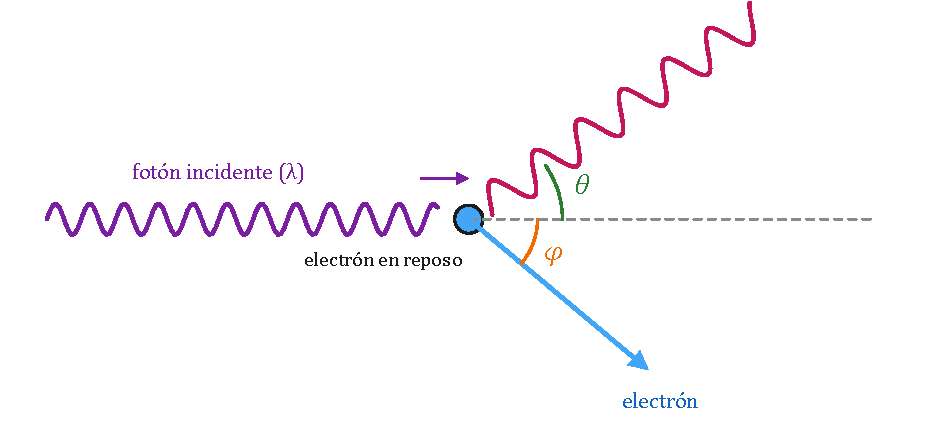
\includegraphics[width=0.62\linewidth]{images/UD7/compton}
    \caption{Efecto Compton: el fotón sale desviado un ángulo \(\theta\) y con mayor longitud de onda.}
    \label{fig:cua-compton}
\end{figure}

\begin{remark}
    El efecto Compton demuestra que el fotón se comporta como una partícula: tiene energía \(E = h\nu\) y también \textbf{cantidad de
    movimiento}, \(p = E/c = h/\lambda\), aunque no tenga masa. El cambio de longitud de onda es apreciable con rayos X (de \(\lambda\)
    muy pequeña), pero no con luz visible.
\end{remark}

\begin{exercise}
    Un fotón de \qty{20}{\kilo\electronvolt} choca con un electrón en reposo y sale desviado \ang{90}. Calcula su longitud de onda antes
    y después del choque y su nueva energía.
    \begin{solu}
        \(\lambda = \dfrac{hc}{E} = \dfrac{6{,}63\cdot 10^{-34}\cdot 3\cdot 10^8}{2\cdot 10^4\cdot 1{,}6\cdot 10^{-19}} = \textcolor{red}{\qty{6.22e-11}{\m}}\);
        \(\lambda' = \lambda + \lambda_C(1 - \cos\ang{90}) = \textcolor{red}{\qty{6.46e-11}{\m}}\).

        \(E' = \dfrac{hc}{\lambda'} = \textcolor{red}{\qty{19.3}{\kilo\electronvolt}}\) \textcolor{blue}{(el electrón se lleva \qty{0.7}{\kilo\electronvolt}).}
    \end{solu}
\end{exercise}

\section{Dualidad onda-corpúsculo. Hipótesis de De Broglie}\label{sec:cua-debroglie}

La luz se comporta como una onda en la propagación, las interferencias o la difracción, y como un chorro de partículas en el efecto
fotoeléctrico o el Compton: tiene un \textbf{comportamiento dual}. En 1924, Louis de Broglie propuso que esta dualidad no es exclusiva
de la luz, sino que vale para toda la materia:

\begin{definition}[Hipótesis de De Broglie]
    Toda partícula en movimiento lleva asociada una onda, cuya longitud de onda depende de su cantidad de movimiento:
    \begin{centeredequation}
        \boxed{\lambda = \dfrac{h}{p} = \dfrac{h}{m\,v}} \label{eq:cua-debroglie}
    \end{centeredequation}
\end{definition}

Si una partícula de carga \(q\) se acelera desde el reposo con una diferencia de potencial \(V\), su energía cinética es \(qV\) y
\(p = \sqrt{2mqV}\), así que \(\lambda = h/\sqrt{2mqV}\).

En 1927, Davisson y Germer observaron la \textbf{difracción de electrones} en un cristal de níquel, con la longitud de onda que predecía
De Broglie. Hoy los microscopios electrónicos aprovechan que la longitud de onda de los electrones es miles de veces menor que la de la
luz visible para ver detalles de tamaño atómico. Para objetos cotidianos, en cambio, \(\lambda\) es tan pequeña que los efectos
ondulatorios son imposibles de observar.

\begin{exercise}
    Calcula la longitud de onda de De Broglie de un electrón con una energía cinética de \qty{150}{\electronvolt} y de una pelota de tenis de
    \qty{60}{\g} que va a \qty{40}{\m\per\second}.
    \begin{solu}
        \textcolor{blue}{Electrón: \(v = \sqrt{2E_c/m} = \qty{7.26e6}{\m\per\second}\).} \(\lambda = \dfrac{h}{mv} = \textcolor{red}{\qty{1.0e-10}{\m}}\)
        \textcolor{blue}{(del tamaño de un átomo: se difracta en los cristales).}

        Pelota: \(\lambda = \dfrac{6{,}63\cdot 10^{-34}}{0{,}06\cdot 40} = \textcolor{red}{\qty{2.8e-34}{\m}}\) \textcolor{blue}{(totalmente inobservable).}
    \end{solu}
\end{exercise}

\subsection{La doble rendija}\label{subsec:cua-young}

En 1801, Thomas Young hizo pasar la luz de una rendija \(S_0\) por dos rendijas muy próximas, \(S_1\) y \(S_2\). Como proceden del mismo
frente de onda, son focos coherentes, y en la pantalla aparecen franjas brillantes y oscuras: la interferencia de la
unidad~2 (figura~\ref{fig:cua-young}). Fue la gran prueba de la naturaleza ondulatoria de la luz.

\begin{figure}[H]
    \centering
    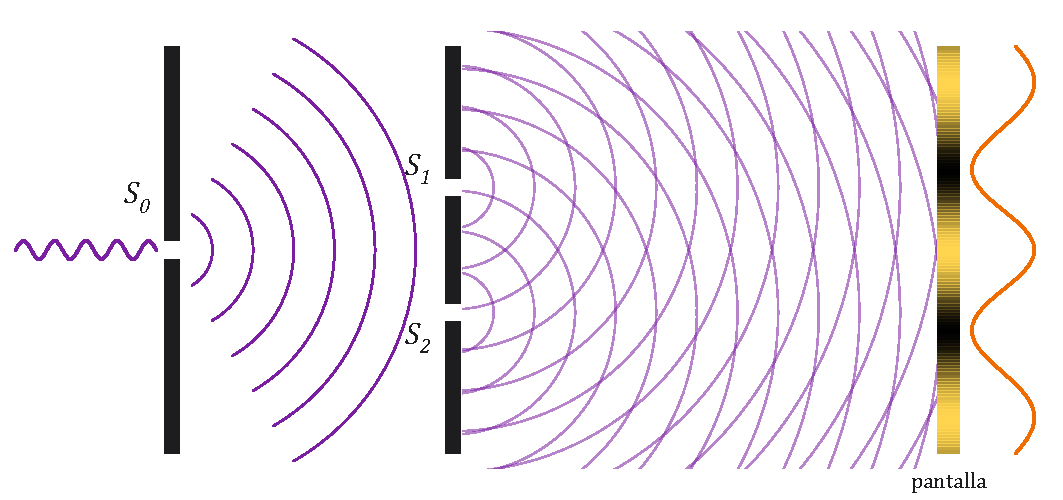
\includegraphics[width=0.75\linewidth]{images/UD7/young}
    \caption{Experimento de la doble rendija. La intensidad en la pantalla (a la derecha) se ha calculado con la diferencia de caminos.}
    \label{fig:cua-young}
\end{figure}

Lo sorprendente es que el experimento funciona igual con \emph{electrones} (y hasta con moléculas grandes). Si se envían de uno en uno,
cada electrón llega a un punto concreto de la pantalla, como una partícula; pero, al acumular miles, aparecen las franjas de
interferencia, como si cada electrón hubiera pasado por las dos rendijas a la vez. Y si se intenta averiguar por cuál pasa, las franjas
desaparecen. La mecánica cuántica no dice dónde llegará cada electrón, solo la \textbf{probabilidad} de que llegue a cada punto.

\section{El principio de incertidumbre}\label{sec:cua-heisenberg}

En física clásica, conociendo con precisión la posición y la velocidad de una partícula se puede predecir su movimiento futuro. En 1927,
Werner Heisenberg demostró que eso es imposible en el mundo cuántico:

\begin{definition}[Principio de incertidumbre de Heisenberg]
    No es posible conocer a la vez, con precisión ilimitada, la posición y la cantidad de movimiento de una partícula. El producto de sus
    incertidumbres cumple:
    \begin{centeredequation}
        \boxed{\Delta x\cdot\Delta p \geq \dfrac{h}{2\pi}} \label{eq:cua-heisenberg}
    \end{centeredequation}
    Una relación análoga liga la energía y el tiempo: \(\Delta E\cdot\Delta t \geq h/2\pi\).
\end{definition}

No es un problema de los aparatos de medida: es una propiedad de la naturaleza. Para observar un electrón hay que iluminarlo, y el fotón
que rebota le cambia la velocidad; cuanto menor sea su longitud de onda (para precisar la posición), mayor será el golpe. La mecánica
cuántica, desarrollada por Heisenberg, Schrödinger y Dirac, describe las partículas con funciones de onda que dan
\textbf{probabilidades}, no trayectorias. Einstein nunca aceptó del todo este carácter probabilista: «Dios no juega a los dados».

\begin{exercise}
    Se conoce la posición de un objeto de \qty{5}{\kg} con una incertidumbre de \qty{0.1}{\mm}. ¿Cuál es la incertidumbre mínima de su velocidad?
    \begin{solu}
        \(\Delta v = \dfrac{h}{2\pi\,m\,\Delta x} = \dfrac{6{,}63\cdot 10^{-34}}{2\pi\cdot 5\cdot 10^{-4}} = \textcolor{red}{\qty{2.1e-31}{\m\per\second}}\):
        \textcolor{blue}{en los objetos macroscópicos el principio no tiene ninguna consecuencia práctica.}
    \end{solu}
\end{exercise}

\begin{exercise}
    Una partícula de \qty{3}{\micro\g} se mueve a \qty{4}{\cm\per\second} y su velocidad se conoce con una incertidumbre del \qty{0.001}{\percent}.
    ¿Cuál es la incertidumbre mínima de su posición?
    \begin{solu}
        \(\Delta v = 0{,}04\cdot 10^{-5} = \qty{4e-7}{\m\per\second}\);
        \(\Delta x = \dfrac{h}{2\pi m\,\Delta v} = \dfrac{6{,}63\cdot 10^{-34}}{2\pi\cdot 3\cdot 10^{-9}\cdot 4\cdot 10^{-7}} = \textcolor{red}{\qty{8.8e-20}{\m}}\).
    \end{solu}
\end{exercise}

\section{Los postulados de la relatividad especial}\label{sec:cua-relatividad}

La otra «nubecilla» era el experimento de Michelson y Morley (1887), que buscaba medir la velocidad de la Tierra respecto del éter, el
supuesto medio en el que se propagaba la luz. El resultado fue nulo: la luz iba igual de rápido en todas las direcciones. En 1905 Einstein
resolvió el problema con dos postulados:
\begin{enumerate}[label=\numberballmDarkTeal]
    \item \textbf{Principio de relatividad.} Las leyes de la física son las mismas en todos los sistemas de referencia inerciales (los
    que se mueven con velocidad constante unos respecto de otros). No existe un sistema de referencia absoluto, ni el éter.
    \item \textbf{Constancia de la velocidad de la luz.} La velocidad de la luz en el vacío, \(c\), es la misma para todos los observadores
    inerciales, sea cual sea el movimiento del foco o del observador.
\end{enumerate}
De estos postulados se deducen consecuencias asombrosas: el tiempo transcurre más despacio para un reloj en movimiento (dilatación del
tiempo), las longitudes se contraen en la dirección del movimiento, nada con masa puede alcanzar la velocidad de la luz, y la masa es una
forma de energía, \(E = mc^2\), que estudiaremos en la próxima unidad.

\paragraph{Espectros atómicos.} Para terminar, una aplicación de la cuantización. Si se analiza con un prisma la luz que emite un gas
calentado, no se obtiene un espectro continuo, sino una serie de líneas de colores: es su \azuln{espectro de emisión}. Si se hace pasar luz
blanca por el gas frío, faltan justo esas mismas líneas: es su \azuln{espectro de absorción}. Cada elemento tiene sus propias líneas, como
una huella dactilar. Bohr las explicó en 1913: los electrones de un átomo solo pueden tener ciertas energías, y al saltar de un nivel a otro
emiten o absorben un fotón de energía \(h\nu = E_2 - E_1\).

\section{Resumen de fórmulas}\label{sec:cua-resumen}

\begin{table}[H]
    \centering
    \caption{Fórmulas principales de la física cuántica}
    \vspace{-5pt}
    \begin{tabular}{@{}lL{10cm}@{}}
        \toprule
        \textbf{Magnitud} & \textbf{Expresión} \\
        \midrule
        Ondas electromagnéticas & \(c = \lambda\nu\), \quad \(c = \qty{3e8}{\m\per\second}\) \\[3pt]
        Ley de Wien & \(\lambda_{\text{máx}}\,T = \qty{2.9e-3}{\m\kelvin}\) \\[3pt]
        Ley de Stefan-Boltzmann & \(I = \sigma T^4\), \quad \(\sigma = \qty{5.67e-8}{\watt\per\m\squared\per\kelvin\tothe{4}}\) \\[3pt]
        Energía del fotón & \(E = h\nu = hc/\lambda\), \quad \(h = \qty{6.63e-34}{\joule\second}\), \quad \(\qty{1}{\electronvolt} = \qty{1.6e-19}{\joule}\) \\[3pt]
        Efecto fotoeléctrico & \(h\nu = W_0 + E_{c,\text{máx}}\), \quad \(W_0 = h\nu_0\), \quad \(eV_0 = E_{c,\text{máx}}\) \\[3pt]
        Efecto Compton & \(\lambda' - \lambda = \lambda_C(1 - \cos\theta)\), \quad \(\lambda_C = \qty{2.43e-12}{\m}\) \\[3pt]
        De Broglie & \(\lambda = h/(mv)\); \quad partícula acelerada: \(\lambda = h/\sqrt{2mqV}\) \\[3pt]
        Heisenberg & \(\Delta x\cdot\Delta p \geq h/2\pi\), \quad \(\Delta E\cdot\Delta t \geq h/2\pi\) \\
        \bottomrule
    \end{tabular}
    \label{tab:cua-resumen}
\end{table}

\section{Prácticas}\label{sec:cua-practicas}

\subsection{Práctica 1: medida de la constante de Planck con LED}\label{subsec:cua-practica-led}

\textbf{Objetivo.} Estimar la constante de Planck midiendo la tensión a la que empiezan a lucir LED de distintos colores.

\textbf{Material.} LED de varios colores (rojo, naranja, amarillo, verde, azul) de longitud de onda conocida, fuente de tensión
regulable, resistencia de protección de unos \qty{1}{\kilo\ohm}, voltímetro, y una caja o tubo oscuro para observar.

\textbf{Fundamento.} En un LED, cada electrón que atraviesa la unión pierde una energía \(eV\) y la emite como un fotón. El LED empieza a
lucir cuando \(eV_u \approx hc/\lambda\), donde \(V_u\) es la tensión umbral.

\textbf{Procedimiento.}
\begin{enumerate}[label=\numberballmDarkTeal]
    \item Monta en serie la fuente, la resistencia y el LED, con el voltímetro en paralelo con el LED.
    \item Sube poco a poco la tensión y anota el valor en el que el LED empieza a emitir luz (obsérvalo dentro del tubo oscuro).
    \item Repite con cada color.
\end{enumerate}

\begin{table}[H]
    \centering
    \caption{Datos de la práctica de los LED}
    \vspace{-5pt}
    \begin{tabular}{@{}C{2.4cm}C{2.4cm}C{2.8cm}C{2.4cm}C{2.8cm}@{}}
        \toprule
        \textbf{Color} & \textbf{\(\lambda\) (\unit{\nm})} & \textbf{\(1/\lambda\) (\unit{\per\m})} & \textbf{\(V_u\) (\unit{\volt})} & \textbf{\(h = eV_u\lambda/c\)} \\
        \midrule
        \rule{0pt}{18pt} & & & & \\ \midrule[0.3pt]
        \rule{0pt}{18pt} & & & & \\ \midrule[0.3pt]
        \rule{0pt}{18pt} & & & & \\ \midrule[0.3pt]
        \rule{0pt}{18pt} & & & & \\
        \bottomrule
    \end{tabular}
    \label{tab:cua-practica}
\end{table}

\textbf{Cálculos.} Representa \(V_u\) frente a \(1/\lambda\). La pendiente de la recta es \(hc/e\); de ella obtén \(h\).

\textbf{Cuestiones.}
\begin{enumerate}[label=\letraminuscula]
    \item Calcula el error relativo respecto al valor \(h = \qty{6.63e-34}{\joule\second}\).
    \item ¿Por qué el LED azul necesita más tensión que el rojo?
    \item ¿Qué relación tiene esta experiencia con el efecto fotoeléctrico?
\end{enumerate}

\subsection{Práctica 2: difracción de un láser en una red}\label{subsec:cua-practica-red}

\textbf{Objetivo.} Comprobar el carácter ondulatorio de la luz y medir la longitud de onda de un puntero láser.

\textbf{Material.} Puntero láser, red de difracción de \(N\) líneas por milímetro (por ejemplo, 300), pantalla, cinta métrica. Un CD
puede hacer de red de reflexión (unas 625 líneas por milímetro).

\textbf{Procedimiento y cálculos.} Haz incidir el láser perpendicularmente sobre la red y mide, en la pantalla situada a una distancia
\(D\), la separación \(x\) entre el máximo central y el primer máximo lateral. La condición de máximo es \(d\sen\theta = \lambda\), con
\(d = 1/N\) y \(\tg\theta = x/D\).

\textbf{Cuestiones.}
\begin{enumerate}[label=\letraminuscula]
    \item Calcula \(\lambda\) y compárala con la que indica el láser.
    \item ¿Qué ocurriría con la separación entre máximos si usaras un láser verde? ¿Y con una red de más líneas por milímetro?
    \item ¿Por qué esta experiencia apoya el modelo ondulatorio y no el corpuscular?
\end{enumerate}
